まずRequestパケットの構造を見てみることにしましょう。Requestパケットは3つの部分にわけられます。第一部分はRequest line(リクエスト行)。第二部分はRequest header(リクエストヘッダ)、第三部分はbody(ボディ)と呼ばれます。headerとbodyの間には空行があり、リクエストパケットの例は以下のようなものです。

\begin{lstlisting}[numbers=none]
GET /domains/example/ HTTP/1.1
//リクエスト行:リクエスト方法 リクエストRUI HTTPプロトコル/プロトコルバージョン
Host:www.iana.org  //サーバのホスト名
User-Agent:Mozilla/5.0 (Windows NT 6.1)
            AppleWebKit/537.4 (KHTML, like Gecko)
            Chrome/22.0.1229.94 Safari/537.4
//ブラウザ情報
Accept:text/html,application/xhtml+xml,
       application/xml;q=0.9,*/*;q=0.8    //クライアントが受け取れるmime
Accept-Encoding:gzip,deflate,sdch //ストリーム圧縮をサポートするか否か
Accept-Charset:UTF-8,*;q=0.5        //クライアントの文字コードセット
//空行、リクエストヘッダとボディを分けるために使われます。
//ボディ、リソースへのリクエストのオプション、例えばPOSTが渡すオプション
\end{lstlisting}

HTTPプロトコルはサーバに対して交互にリクエストを送る方法が定義されています。基本は四種類。GET,POST,PUT,DELETEです。ひとつのURLアドレスはひとつのネットワーク上のリソースを描写しています。またHTTPの中のGET, POST, PUT, DELETEはこのリソースの検索、修正、増加、削除の4つの操作に対応しています。よく見かけるのはGETとPOSTです。GETは一般的にリソースの情報を取得/検索するために用いられ、POSTはリソース情報を更新するために用いられます。

fiddlerパケットキャプチャを通して下のようなリクエスト情報を見ることができます。

\begin{figure}[H]
  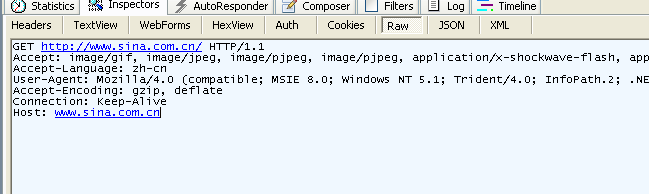
\includegraphics[width=14cm]{3.1.http.png}
   \label{図3.4}
   \caption{fiddlerがキャプチャしたGET情報}
\end{figure}


\begin{figure}[H]
  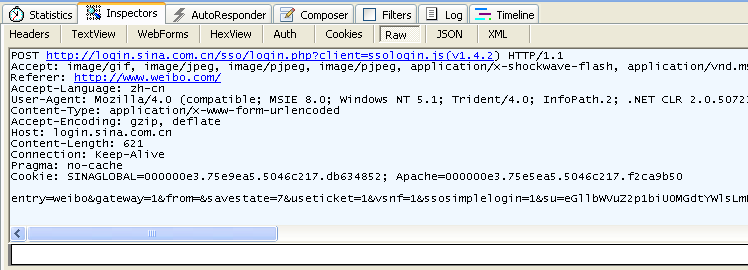
\includegraphics[width=14cm]{3.1.httpPOST.png}
   \label{図3.5}
   \caption{fiddlerがキャプチャしたPOST情報}
\end{figure}

GETとPOSTの区別を見てみましょう。

\begin{enumerate}
  \item GETリクエストのボディが空であることがわかります。POSTリクエストにはボディがあります。
  \item GETが入力するデータはURLの後に置かれます。?によってURLと渡すデータを分割します。オプションの間は\&で繋ぎます。例えばEditPosts.aspx?name=test1\&id=12345。POSTメソッドは入力するデータをHTTPパケットのBodyの中に置きます。
  \item GETが入力するデータの大きさには制限があります。(ブラウザのURLに対する長に制限があるためです。)またPOSTメソッドで入力するデータには制限がありません。
  \item GETメソッドで入力されたデータはセキュリティの問題を引き起こします。例えばログイン画面があったとして、GETメソッドでデータを入力した場合、ユーザ名とパスワードはURL上にあらわれてしまうことになります。もしページがバッファリングされていたり他の人によっがこのマシンにアクセスすることができれば、ヒストリログからこのユーザのアカウントとパスワードを取得することができてしまいます。
\end{enumerate}


